%! Date = 2/23/24

\section{Background}\label{sec:Background}
%\begin{table}[!h]
%    \centering
%    \begin{tabular}{ll}
%        \toprule
%        \textbf{Notation} & \textbf{Description} \\
%        \midrule
%        $L$ & Number of layers in $M$ \\
%        $i$ & Interval of an MoE layer, $L\equiv 0\:(\mathrm{mod}\: i)$ \\
%        $W$ & World Size \\
%        $b$ & Micro batch processed in each step  \\
%        $s$ & Sequence (or context) length \\
%        $h$ & Embedding dimension or hidden size \\
%        $k$ & Subset of experts, per token, selected by the Gate \\
%        \bottomrule
%    \end{tabular}
%    \caption{Description of Notation}
%    \label{tab:notation}
%\end{table}
%\begin{figure}[!h]
%    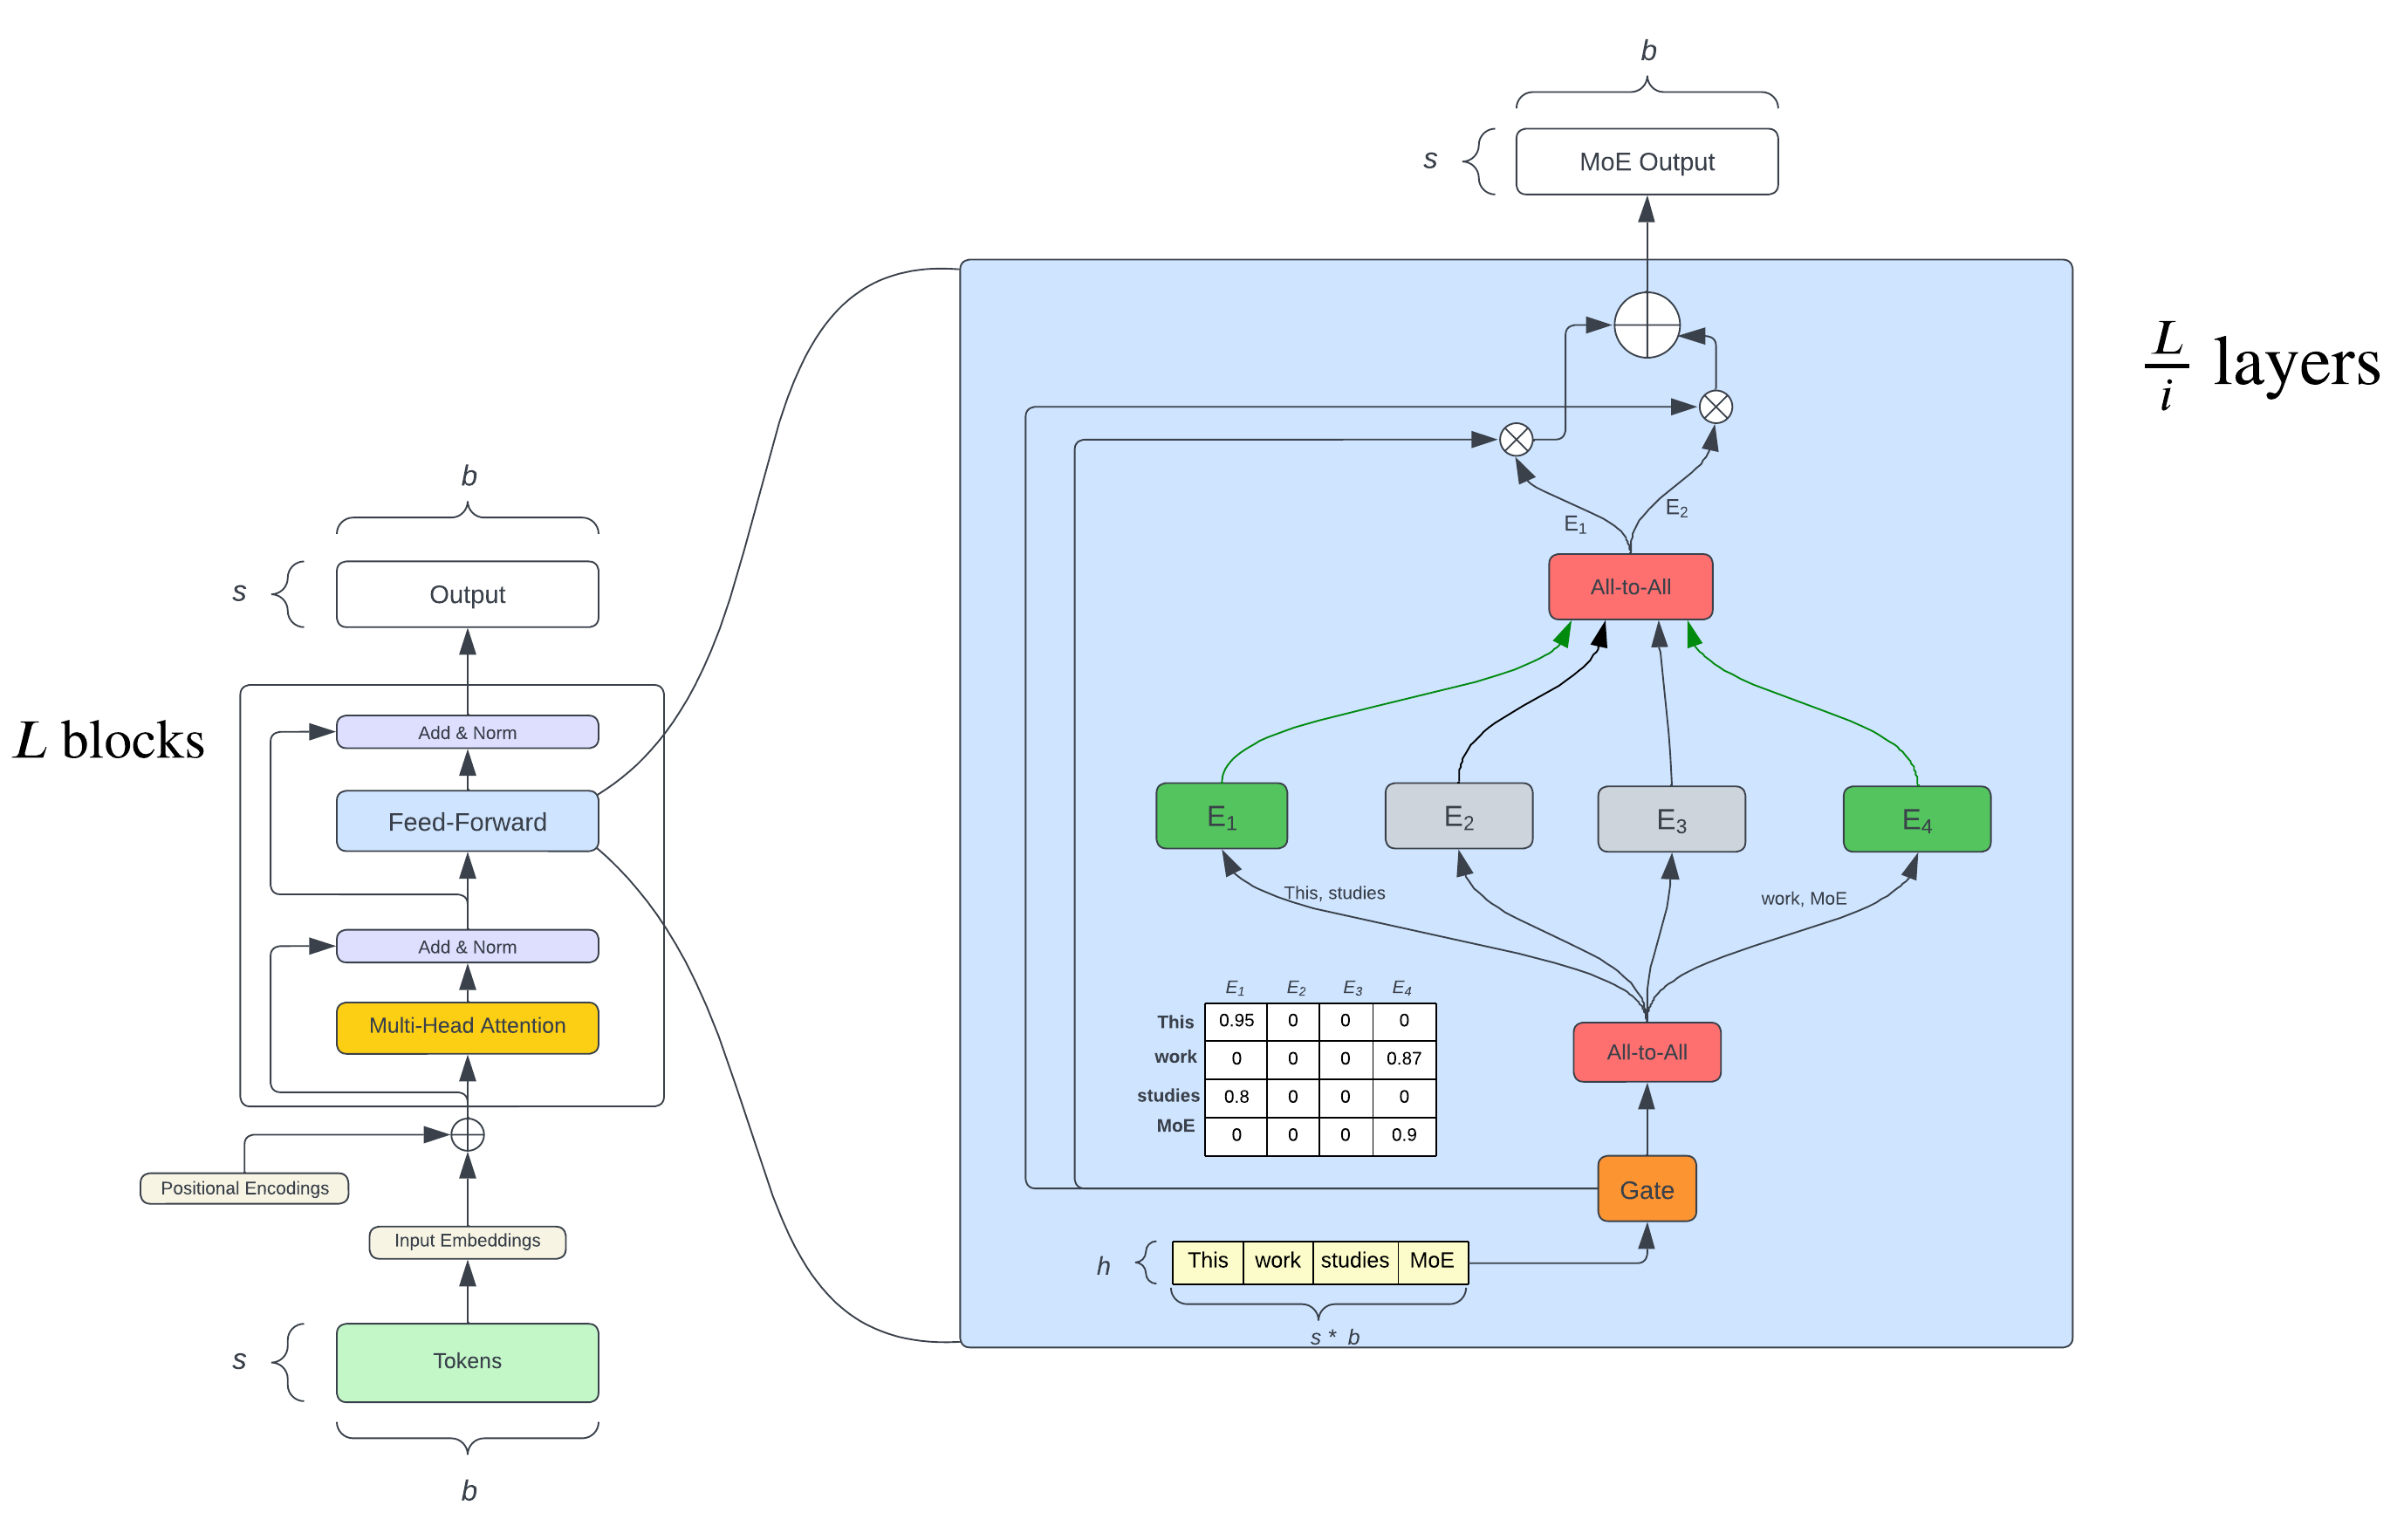
\includegraphics[width=0.75\linewidth]{images/MoE}
%    \caption{Distributed MoE Layer as described in~\cite{DBLP:journals/corr/abs-2006-16668}}
%    \label{fig:moeLayer}
%\end{figure}
%\begin{figure}[!h]
%    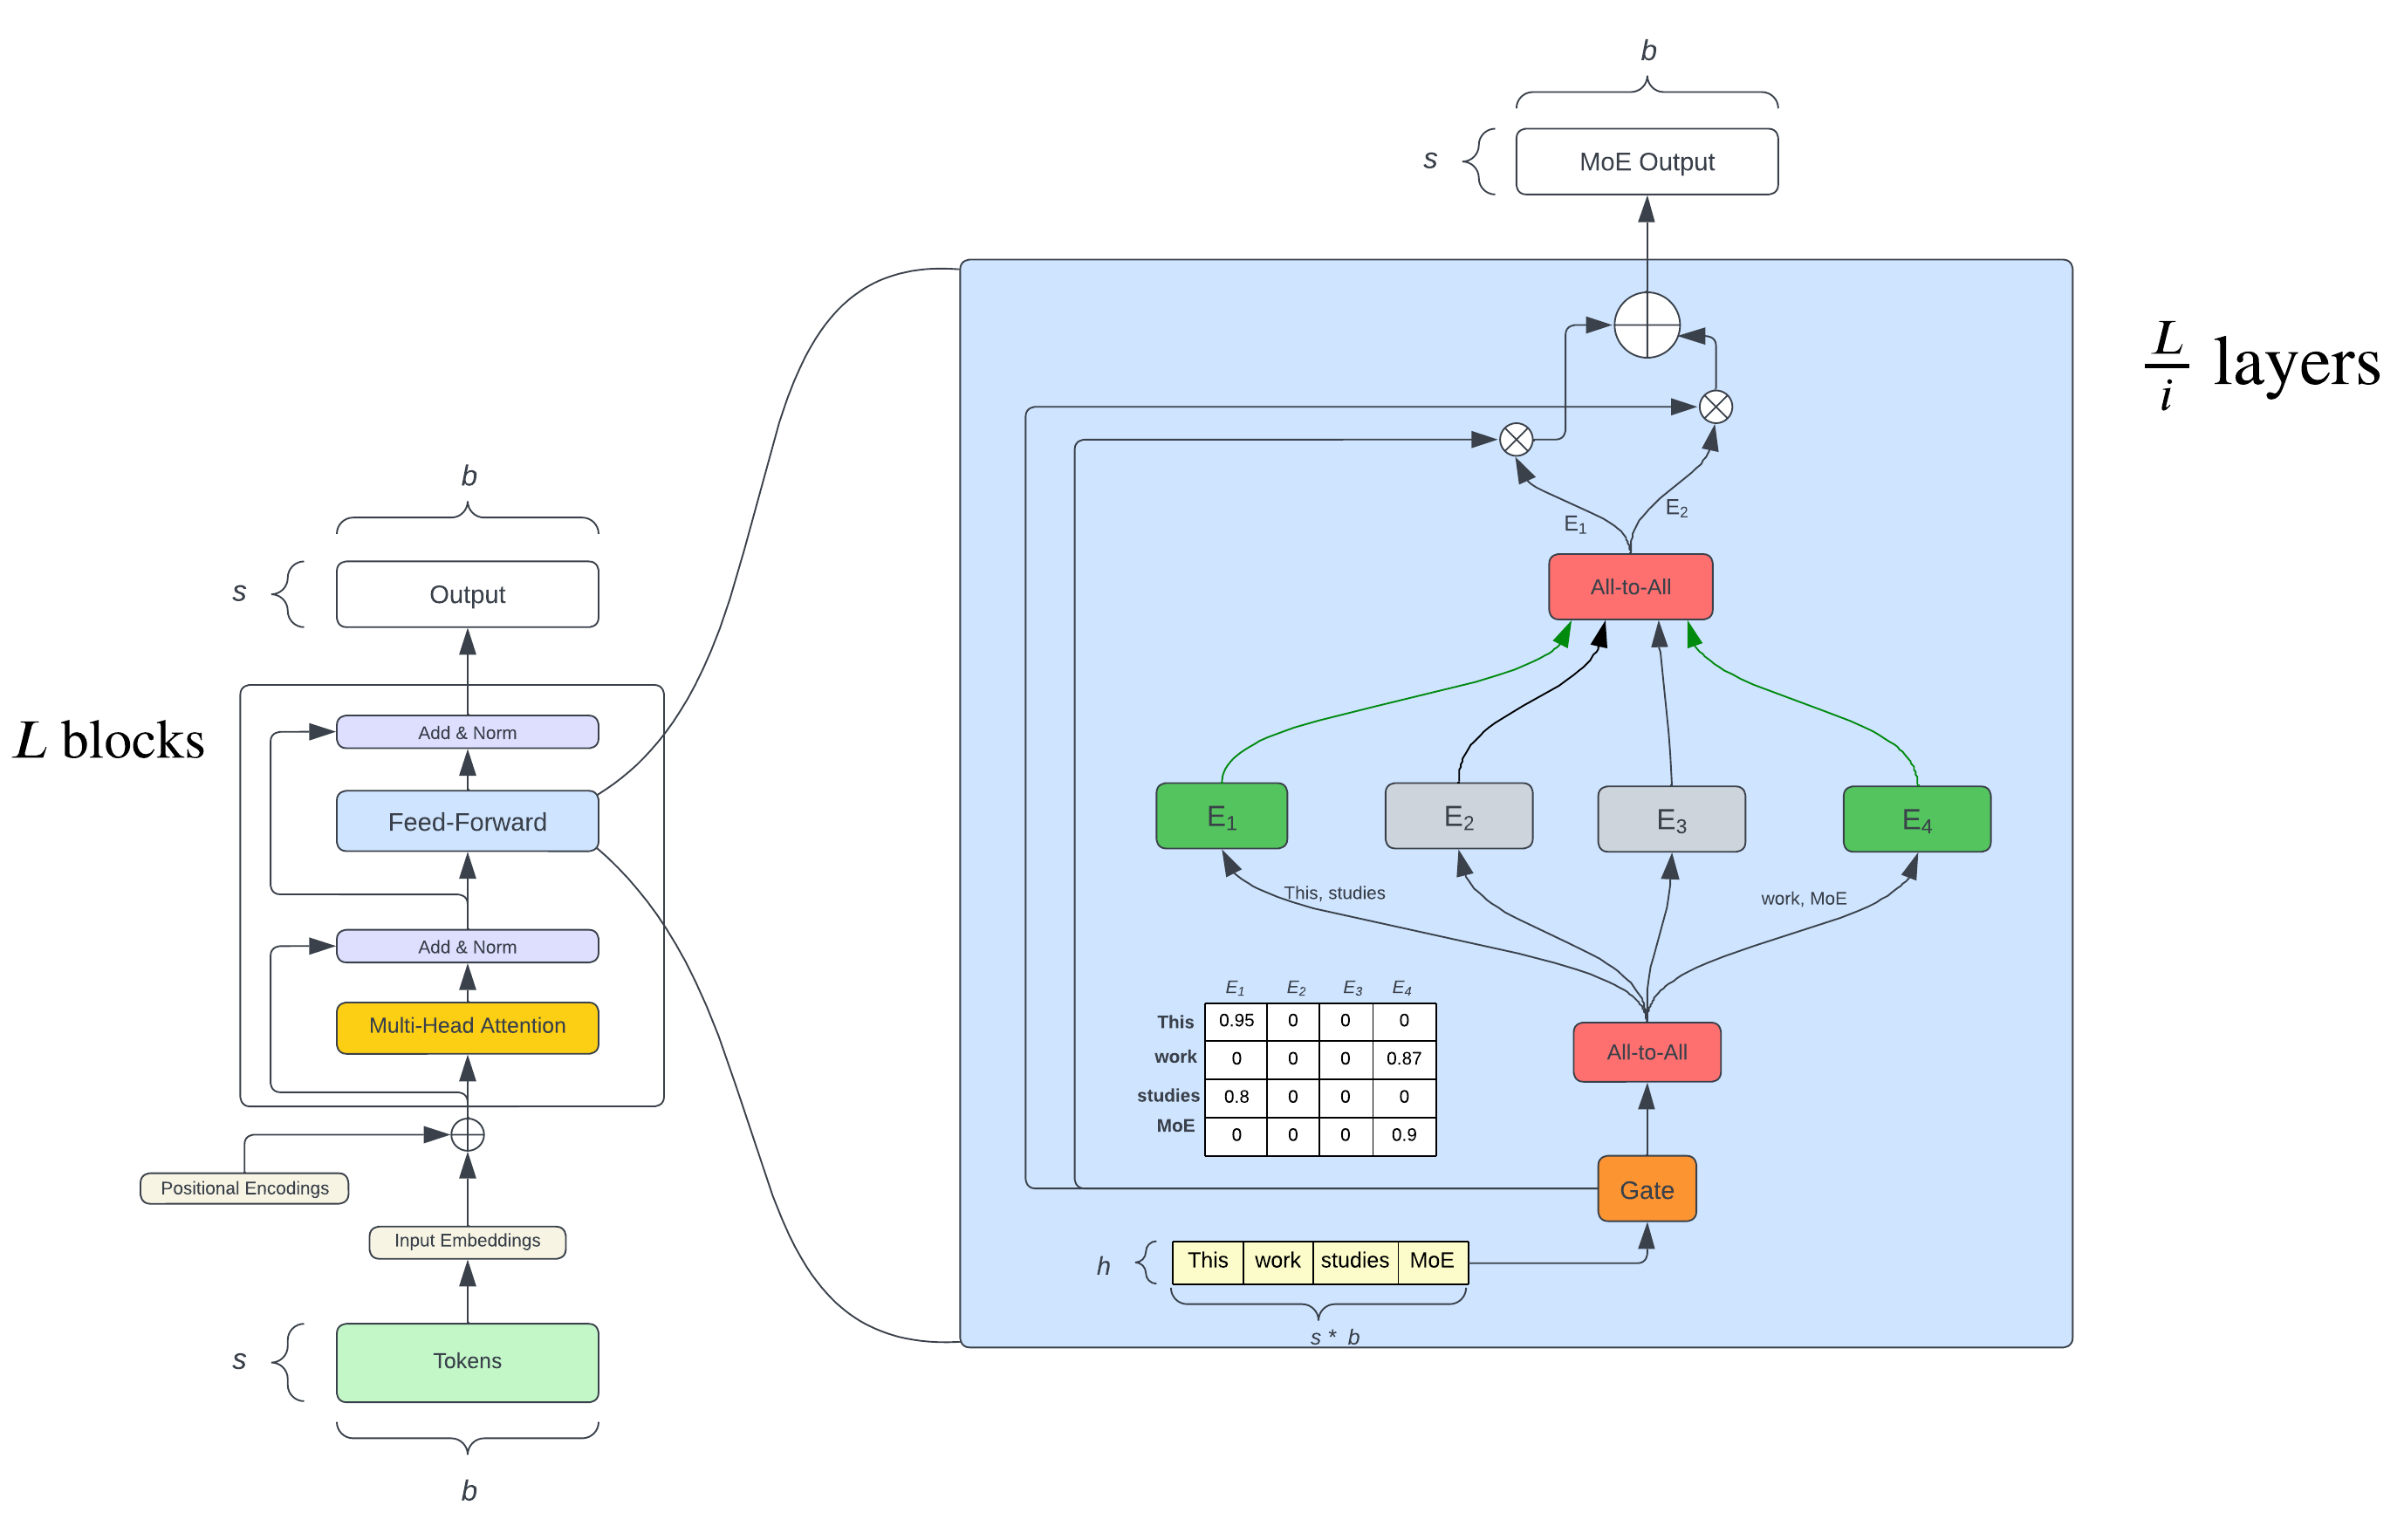
\includegraphics[width=0.75\linewidth]{images/MoE}
%    \caption{Distributed MoE Layer as described in~\cite{DBLP:journals/corr/abs-2006-16668}}
%    \label{fig:moeLayer}
%\end{figure}
Current DMoE practice, introduced by Lepikhin et al.,~\cite{DBLP:journals/corr/abs-2006-16668},
involves sharding the experts and gate networks across workers.
Termed \emph{expert parallelism}, this placement strategy as implemented in practice entails
each worker hosting $\geq 1$ expert such that $W \equiv 0 \: (\mathrm{mod \:} |X|)$.
In performing and reverting tensor re-sharding from sequence to expert dimensions,
expert parallelism requires two executions \emph{per} MoE layer of the communication primitive~\verb|All-to-All|.
Define $A_s$ as the total executions of \verb|All-to-All|~necessary
for a single training step: forward and backward passes.
We highlight
\footnote{The derivation is evident and left as an exercise.}\footnote{Note that $i \in \{1, 2\}$
    from~\cite{DBLP:journals/corr/abs-2101-03961,mixtral8x7B, DBLP:journals/corr/abs-2006-16668}}
that $A_s = \frac{3\cdot L}{i}$, where $L$ is the number of layers and $i$ the MoE layer frequency.
\textbf{Note} that for Distributed Data Parallelism (DDP), an \emph{iteration} comprises $\frac{B}{W\cdot b} \geq 1$
steps~\footnote{Typically $b = 4$ and from
\cite{DBLP:journals/corr/abs-2005-14165} $B \in \{256, 512, 1034, 1536\}$}.
Thus, we have that $A_s = \frac{3 \cdot B\cdot L}{i \cdot W \cdot b}$, where $b$ and $B$ are the mini and global
batch sizes, respectively.
In isolating communication bottlenecks, we use only DDP and expert parallelism in this work.
%\subsection{Empirical Observations}\label{subsec:empirical-observations}
%We further motivate the severity of communication bottlenecks in DMoE from ground-truth measurements of distributed
%training within the Azure NDv2 and the Perlmutter supercomputer~\cite{perlm}.
%The former is a single-node of 8 V100s while the latter comprises 1792 nodes, each hosting 4 A100s.
%We refer the reader to ~\cite{azure, perlm} for more specifications on both systems.
%We develop~\footnote{Code available \href{https://github.com/osayamenja/Megatron-DeepSpeed}{here}}
%a fork of Megatron-DeepSpeed~\cite{megatron-deepspeed}
%and train a GPT-3 MoE model with 350M parameters on a single shard (9B tokens)
%of the copyright-compliant dataset~\verb|monology/pile_uncopyrighted| from Hugging Face\footnote{Link}.
%Finally, we perform profiling using the low-overhead,
%state-of-the-art CUDA profiling systems~\cite{10.1145/3578244.3583736}:
%NSight Systems~\cite{nsys}, which provides access to \emph{all} CUDA Profiling Tools Interface (CUPTI)
%application tracing and kernel-profiling metrics~\cite{cupti}.
%Specifically, the number of profiled kernels is as follows:
%    {\footnotesize \[\sum_{n=1}^{2}\gamma_n \cdot \kappa_n = 23928, \> where\> \gamma \in \{8, 4\},\> \kappa \in \{2010, 1962\}\]}
%%In Figure ~\ref{fig:perfvar}, for each iteration we sample the slowest kernel execution time across
%%\begin{figure}[!h]
%%    \begin{subfigure}{.5\linewidth}
%%        \centering
%%        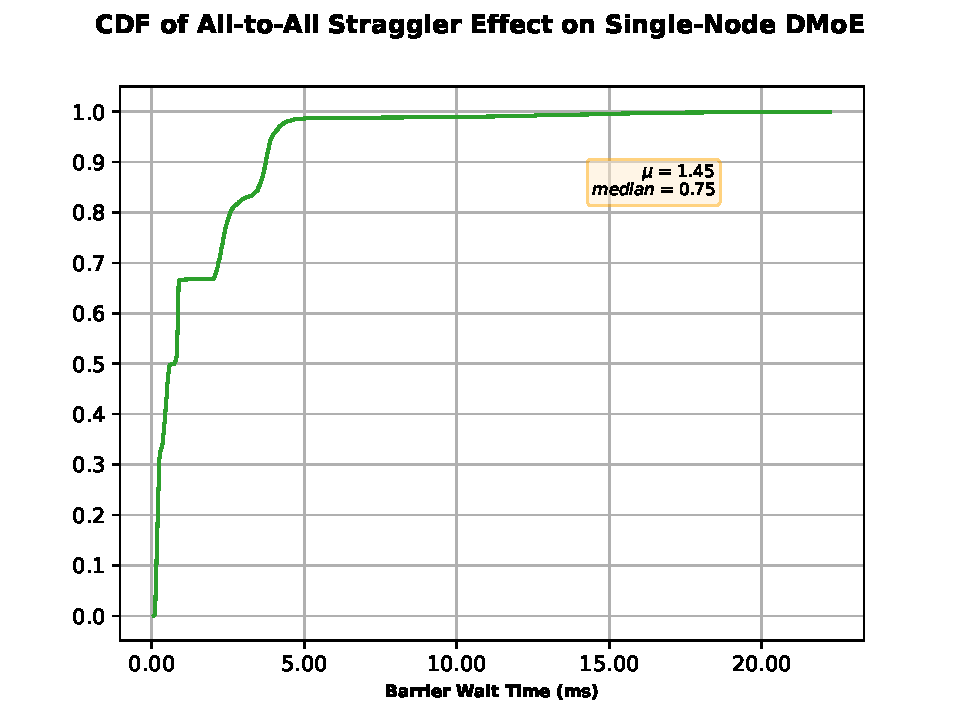
\includegraphics[width=0.8\linewidth]{images/barrier_s}
%%        \caption{Barrier Times on \\ NDv2}
%%        \label{singleecdf}
%%    \end{subfigure}\hfill % <-- "\hfill"
%%    \begin{subfigure}{.5\linewidth}
%%        \centering
%%        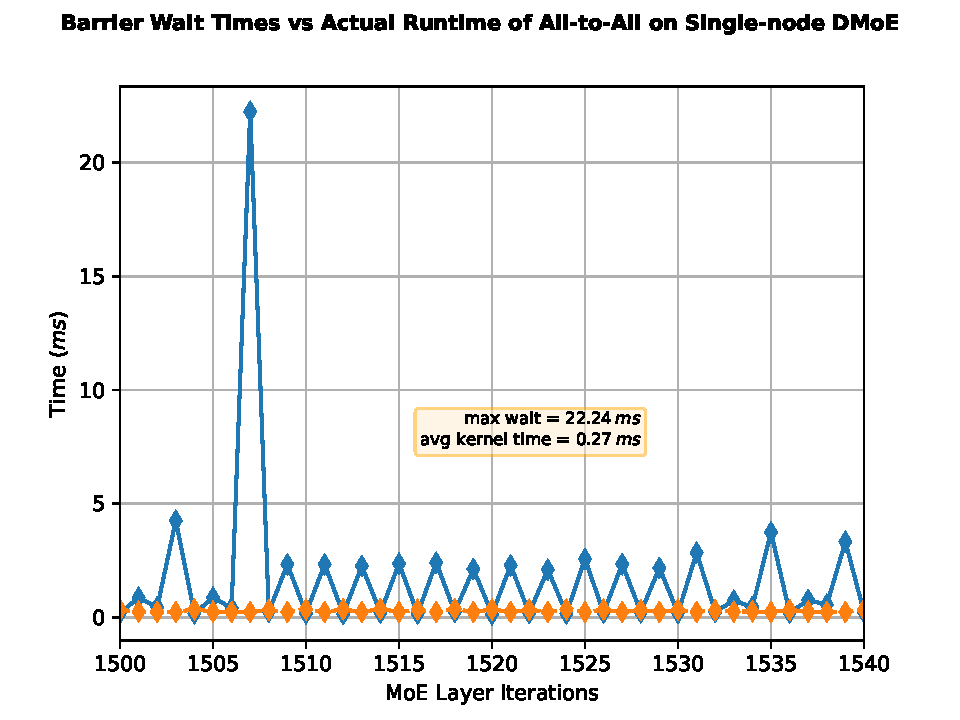
\includegraphics[width=0.8\linewidth]{images/s_distribution}
%%        \caption{Barrier vs. Actual Kernel Time on NDv2}
%%        \label{singlebarriers}
%%    \end{subfigure}
%%
%%    \medskip % create some *vertical* separation between the graphs
%%    \begin{subfigure}{.5\linewidth}
%%        \centering
%%        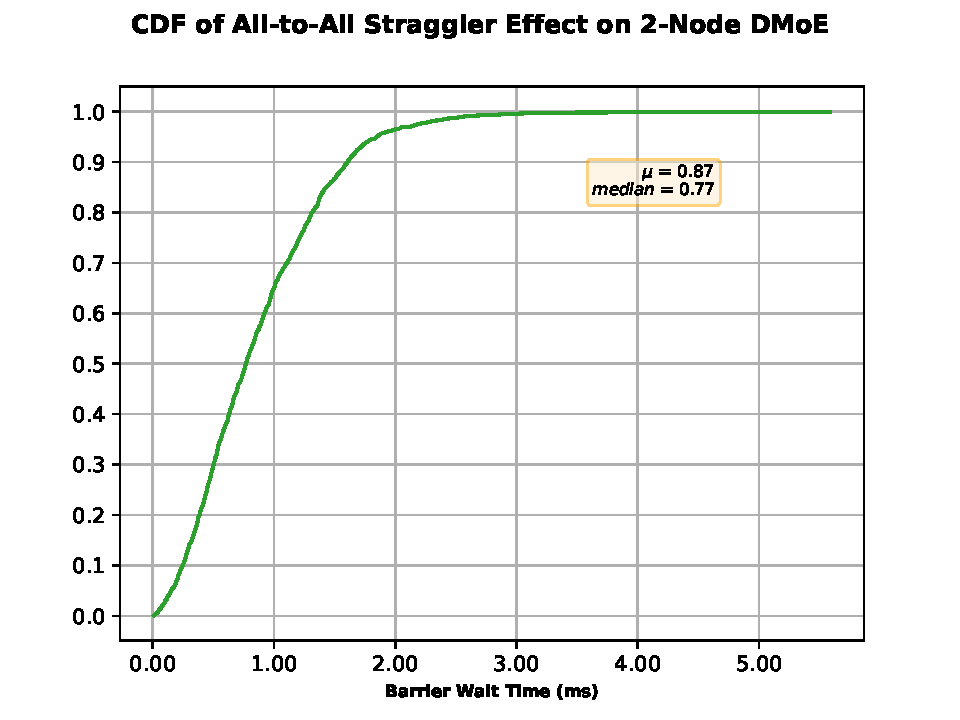
\includegraphics[width=0.8\linewidth]{images/barrier_m}
%%        \caption{Barrier Times on \\ Perlmutter}
%%        \label{multibecdf}
%%    \end{subfigure}\hfill % <-- "\hfill"
%%    \begin{subfigure}{.5\linewidth}
%%        \centering
%%        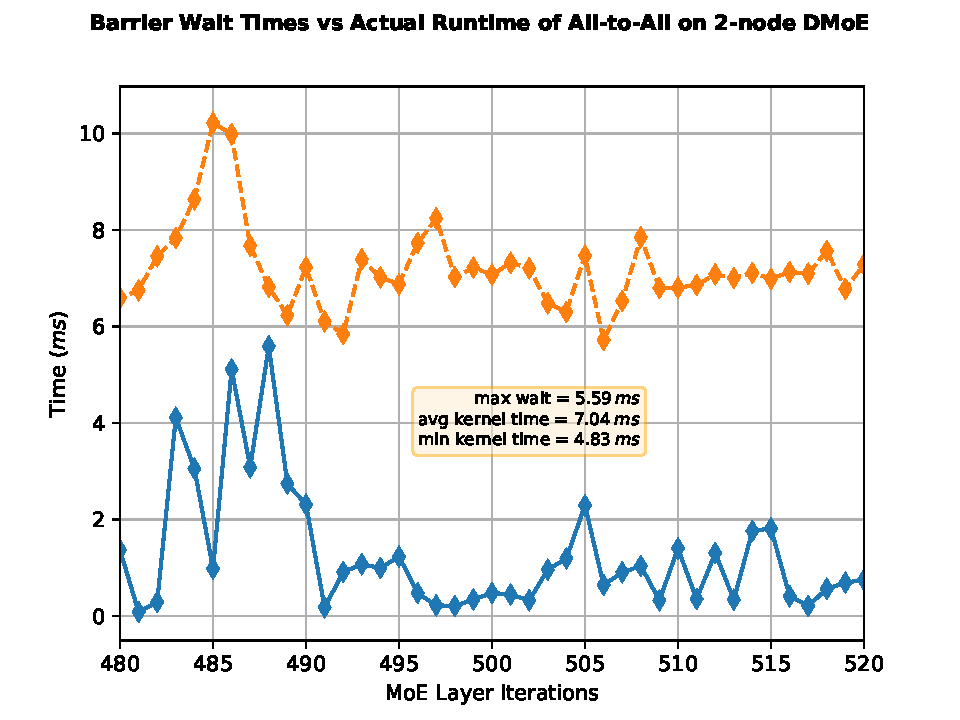
\includegraphics[width=0.8\linewidth, keepaspectratio]{images/m_distribution}
%%        \caption{Barrier vs. Actual Kernel Time on Perlmutter}
%%        \label{multibarriers}
%%    \end{subfigure}
%%
%%    \caption{\small\emph{All-to-All} barrier times in DMoE Training.
%%    Note that the data transfer amount is static at \textbf{2MB} from GPU to
%%    every other GPU for every communication kernel shown. All communication CUDA kernels
%%    also had complete bandwidth and GPU occupancy as they were not overlapped with other kernels.}
%%    \label{fig:perfvar}
%%\end{figure}
%%Figure~\ref{singlebarriers} makes it clear that the interconnect within an NVLink-connected single-node
%is not the bottleneck but rather, the synchronization delay due to the implicit barrier of SOTA~\verb|All-to-All|.
%Observe that on average $\geq 1$ idles for time equivalent to computing \textbf{6}~\verb|All-to-All|
%communication kernels.
